\section{The ATLAS Detector}

The ATLAS detector \cite{:1999fq}, shown in figure \ref{ATLAS}, is a large, multi-purpose detector designed with the ability to discover a variety of different physics signals during the lifetime of the LHC. To do this, the detector is comprised of a number of sub-detectors each of which which fulfills a specific function. 
At the centre of ATLAS, surrounding the interaction point, is the inner detector (ID).
% which comprises the 
%pixel detector, semi-conductor tracker (SCT) and transition radiation tracker (TRT). 
The ID provides tracking, vertex reconstruction, transverse momentum measurement and some level of particle identification. 
Surrounding the ID are the electromagnetic and hadronic calorimeters, which provide energy and position measurement for all incident photons, electrons and hadrons. On the outside of ATLAS is the muon spectrometer, which provides muon tracking and momentum reconstruction.

The coordinate system used by the ATLAS detector defines the origin to be at the interaction point and the $z$ direction to be along the beam line \cite{:1999fq:Chapter1}. Pseudo-rapidity, $\eta$, is defined as 
\begin{equation}
\eta = -\ln\tan\left(\frac{\theta}{2}\right)
\end{equation}
where $\theta$ is the angle with respect to the $z$ axis. The transverse energy, $E_T$, and transverse momentum, $p_T$, of an object are also defined relative to the $z$ axis by
\begin{equation}
E_T = E\sin\theta \quad \textrm{ and } \quad p_T=p\sin\theta
\end{equation}
where $E$ and $p$ are the energy and momentum of the object in question.
The azimuthal angle, $\phi$, in the transverse plane is defined to be zero in the $x$ direction which points to the centre of the LHC ring. Finally, there is the length used by detector elements covering the azimuthal direction, defined as $R_{\phi} =R\phi$, where R is the radial distance to the beam line.
%In the transverse plane, the positive x direction is defined to point at the centre of the LHC ring, the positive y direction defined to point upwards. 
%point out rapidity and R_{\phi}
\begin{figure} [t]
\centering
    	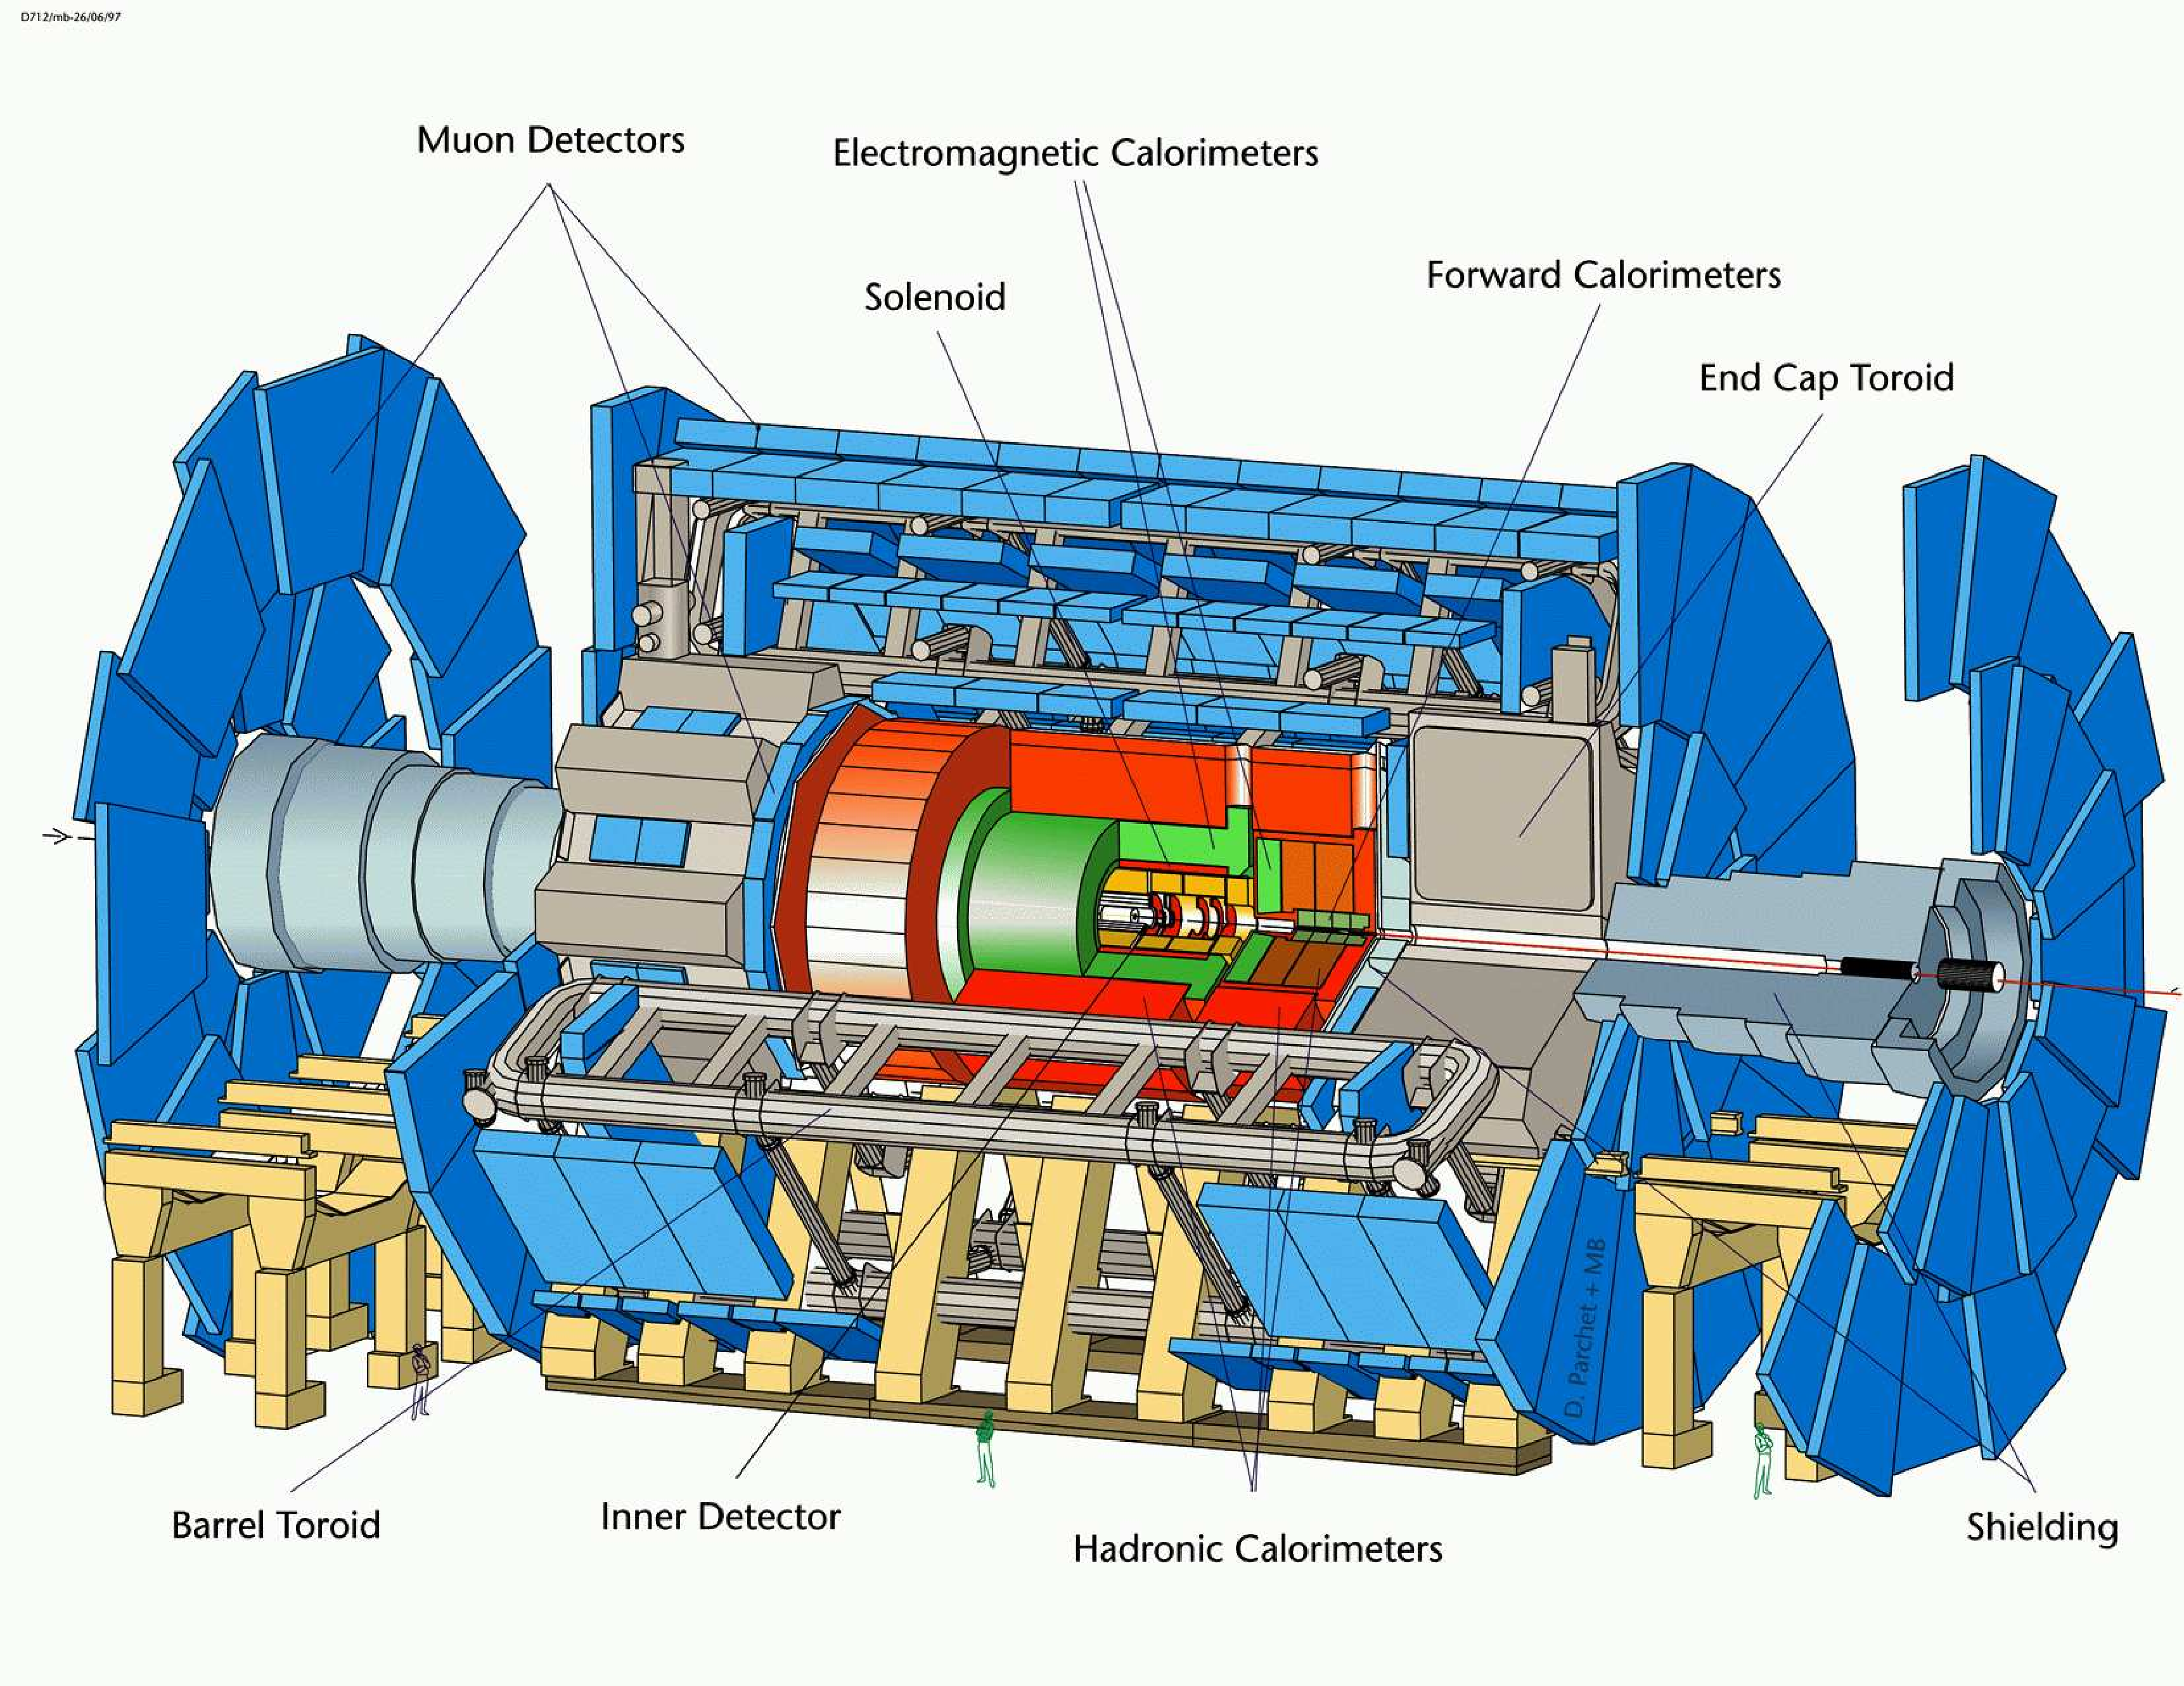
\includegraphics[width=\textwidth]{Diagrams/atlas.eps}
\caption[The ATLAS Detector]{The ATLAS detector \cite{:1999fq}.\label{ATLAS}}
\end{figure}

\subsection{The Inner Detector}

The ID \cite{:1999fq:Chapter1,:1999fq:Chapter3} comprises three sub-detectors covering the pseudo-rapidity range $|\eta| < 2.5$. 
%and is shown in figure \ref{InnerDetector}.  
 The detector nearest the beam is the pixel detector, which is surrounded by the semi-conductor tracker (SCT). The outermost detector is the transition radiation tracker (TRT). Each of these sub-detectors is split into three main components. One is a barrel region which is cylindrical about the beam line with the interaction point at the centre. The other two are endcap regions either side of the interaction point.

%The pixel detector and the SCT are made from silicon. A charged particle passing through the silicon creates electron-hole pairs and a bias voltage across the silicon causes the charges to drift to a readout. If the amount of charge produced is greater than a threshold value then a particle hit is recorded. The TRT is based on straw detector technology. The straws are filled with gas, and a particle traversing the gas causes ionisation. The electrons drift toward a wire readout in the centre of the straw, due to a bias voltage. A particle hit is defined in a similar way to the silicon detectors using a threshold of collected charge.

The pixel detector and the SCT are made from silicon. A charged particle passing through the silicon creates electron-hole pairs and a bias voltage across the silicon causes the charges to drift to a readout electrode. If the amount of charge produced is greater than a threshold value then a particle hit is recorded.
% The pixel detector 

The pixel detector is granular and segmented into pixels of 50~$\mu$m~$\times~$300~$\mu$m. A pixel module consists of 61440 pixels in a 21.4~mm~$\times$~62.4~mm rectangle. In the barrel region, the longer edge of each module is aligned in the $z$ direction and the shorter edge in $R_{\phi}$. The barrel consists of three layers of modules, with each layer providing coverage of $|\eta| < 1.7$ and complete coverage in azimuth. The granularity of the pixels allows precise measurements in $R_{\phi}$ and $z$, with a resolution of 12~$\mu$m and 66~$\mu$m respectively.
%The barrel layers cover the radial region of 4-11cm from the beam. 
Each pixel end-cap consists of five disks of modules covering the pseudo-rapidity range $1.7<|\eta|<2.5$. The position resolution is 12~$\mu$m in $R_{\phi}$ and 77~$\mu$m in $R$.

%The resolution in the position measurement of the pixel detector is 12$\times$66$\mu$m in barrel and 12$\times$77$\mu$m in the end cap disks.
%pixel based on silicon semi conductor technology. charged particle passing through causes electron hole pairs in the semi conductor. A voltage bias collects the charge.
%pixels are segmented in rphi and z.
% individual pixel is 50um x 300um in rphi,z. A module 21.4x62.4mm (61440 pixels). barrel (eta<1.7) has 3 layers, the first starting 4cm from the beam. 5-end cap disks (1.7<eta<2.5) - nearest 11cm radii from beam. The resolution in the measurement is 12x66um in barrel and 12x77um in the end cap disks.

% The silicon tracker
The SCT is made of single sided p-on-n silicon microstrip detectors which have dimension 6.36~$\times$~6.40 cm$^2$ (in the barrel region). Each detector consists of 768 strips of 80~$\mu$m pitch.
% In the barrel region ($|\eta|<$), 768 microstrips are combined into units of 6.36$\times$6.40cm. 
A module consists of four of these detectors, which are wire bonded in pairs to give a length of 12.8~cm. These pairs are then glued back to back at a crossing angle of 40~mrad. This allows precision measurement in one direction, using the granularity provided by the microstrip width, and another measurement perpendicular to the strips using small angle stereo. In the barrel ($|\eta|<1.4$), there are 4 layers of modules which are arranged so that the strips offer segmentation of the $R_{\phi}$ direction. This results in a resolution in $R_{\phi}$ of 16~$\mu$m and the small angle stereo gives a $z$ measurement accurate to 580~$\mu$m. 

The two SCT end-caps each consist of nine disks covering the range $1.4<|\eta|<2.5$. The end-cap modules are constructed in the same way as the barrel modules. However, the microstrips themselves are tapered and there are three sizes of module covering the inner, middle and outer regions of the disk. The modules are aligned on the disks so that one set of strips is in the radial direction, again giving precision measurements in the $R_{\phi}$ direction. The resolution of the end-cap measurements in ($R_{\phi}$, $R$) is the same as the barrel measurements in ($R_{\phi}, z$).
%  barrel : 4 layers of modules. end-cap is 9 disks of modules. Each module has 2 p on n silicon microstrip detectors at a crossing angle of 40mrad. In barrel, each detector is 6.36x6.40cm with 768 strips of 80um pitch. precision measurements in the Rphi direction gives 16um resolution. Small angle stereo gives the z measurement to a resolution of 580um. Are we sure how the small angle stereo works?
% The TRT

The TRT is based on straw detector technology. The straws are filled with gas (70\% Xe, 27\% CO$_2$, 3\% O$_2$) and a charged particle traversing the gas causes ionisation. The electrons drift toward a wire readout in the centre of the straw, due to a bias voltage. A particle hit is defined in a similar way to the silicon detectors using a threshold of collected charge.
The TRT is made of straws 4~mm in diameter and up to 144~cm long. The barrel section ($|\eta|<0.7|$) has 50000 straws, aligned lengthways in the $z$ direction. The end-cap wheels have 320000 radial straws, which are arranged in 18 wheels per end-cap and cover the pseudo-rapidity region $0.7<|\eta|<2.5$. Drift time measurements result in a resolution of 170~$\mu$m per straw. A charged particle passing through the TRT gives typically 36 hits per track.

Radiator material is placed between the straws. Particles with $\beta\gamma \geq 1000$ emit transition radiation photons at the radiator-straw boundary. The emitted radiation is absorbed by the xenon and results in more ionisation than just the initial particle alone. The TRT uses a second, higher threshold to determine whether the hit consists of a particle plus transition radiation. This mechanism allows electron-pion separation in the momentum range $p < 100$~GeV. 

 %because electrons emit transition radiation and pions do not. 
% Above this $p_{T} limit$, the rise of ionisation with $B^2$ causes the separation
%stuff here on trans rad
%i have no idea how this works.
%As electrons traverse the TRT, they emit transition radiation as they pass between straws. The gas mixture in the straws contains Xenon, which is ionised by the transition radiation photons. A second thres

%straw detectors-
%particles ionise the gas to form electron ion pairs. A bias voltage causes the electrons to drift to a sense wire. Each straw is 4mm in diameter and 144cm long with 30um sense wire. Each straw is divided into 2 at centre to reduce occupancy. barrel has 50000 straws. end cap 320000 radial straws arranged in 18 wheels in each cap. Drift time measurement results in resolution of 170um per straw.
%typically 36 hits per track at LHC
%TRT also gives some electron id by detecting photons created as electrons travel through straw-gap-straw boundaries.
%the magnet effects.

The ID is surrounded by a superconducting central solenoid magnet which provides a 2~T magnetic field in the $z$ direction. The central solenoid is kept at 4.5~K and shares the same vacuum vessel as the electromagnetic barrel calorimeter. The charged particles bend in the presence of the magnetic field and the transverse momentum of the particle can be obtained from the radius of curvature of the track. The large number of track hits in the TRT, coupled with the precision measurements of the silicon detectors, result in excellent reconstruction of particle pseudo-rapidity, azimuth, impact parameter ($d_0$) and vertex identification ($z_0$). The resolution of reconstructed muon track parameters, obtained from full simulation \cite{:1999fq:Chapter3}, are:
\begin{eqnarray} \label{trackrec}
\sigma\left(\frac{1}{p_T} \right) & = & 0.36 + \frac{13}{p_T\sqrt{\sin\theta}} \quad(\text{TeV}^{-1})  \nonumber \\
%\qquad 
\sigma\left(\phi \right) & = & 0.075 + \frac{1.8}{p_T\sqrt{\sin\theta}} \quad(\text{mrad}) \nonumber \\
%\nonumber
%\vspace{0.1cm}
%\end{equation*}
%\begin{equation*}
\sigma\left(\cot\theta\right) & = &  \left(0.7 +  \frac{2.0}{p_T\sqrt{\sin^{3}\theta}}\right)\times10^{-3} \nonumber \\
%\qquad
\sigma\left(d_0\right) & = & 11 + \frac{73}{p_T\sqrt{\sin\theta}} \quad (\mu\text{m}) \nonumber \\
%\vspace{0.1cm}
%\end{equation*}
%\begin{equation}\label{trackrec}
\sigma\left(z_0\right) & = & 87 + \frac{115}{p_T\sqrt{\sin^3\theta}} \quad (\mu\text{m}).
%\vspace{0.1cm}
\end{eqnarray}
Pions and electrons are less well measured. Pions have a probability of undergoing a nuclear interaction, which causes tails in reconstructed track parameters. This problem is removed by the standard track quality cuts which are \cite{:1999fq:Chapter3}: at least nine precision hits in the silicon detectors, at least two pixel hits - with one in the inner layer - and a transverse impact parameter less than 1~mm.  The effect of these track quality requirements is to reduce the efficiency of pion track reconstruction, but results in similar resolutions as equation \ref{trackrec}. Electrons on the other hand, emit bremsstrahlung
radiation which leads to a broadening of the smeared distributions of 1/$p_T$, $d_0$ and $\phi$.

\subsection{The Calorimeters}

Calorimeters measure the total energy of particles by complete absorption. The two ATLAS calorimeters \cite{:1999fq:Chapter1,:1999fq:Chapter4,:1999fq:Chapter5} use alternating sheets of material to repeatedly sample the energy. The first type of material causes the particles to shower into a number of secondary particles. The second type of material forms the active part of the detector, which absorbs and measures some of the energy of the produced particles. This process is repeated in many layers until all of the energy is absorbed. 
% differnce in types of showers. - allow differnt calorimeters..shower shapes.

The electromagnetic calorimeter (EM) uses a lead/liquid argon combination to measure the energy of photons and electrons. In the presence of heavy nuclei, electrons emit bremsstralung photons; photons on the other hand split into an electron-positron pair. Thus an incident electron or photon results in a shower of new particles when passing through the lead layer.
%Lead is used in this process due to a high atomic number which results in a short radiation length. 
The electrons produced in the shower cause ionisation in the liquid argon (LAr) and the charge is collected on copper electrodes.

The barrel EM calorimeter covers the region $|\eta|<1.475$ and the end-caps cover $1.375 < |\eta| < 3.2$. However, in the pseudo-rapidity region $|\eta| < 1.8$, the EM calorimeter is preceded by a presampler, which is a just a layer of liquid argon (LAr). The reason for this is that the material preceding the calorimeter can cause showering and the presampler corrects for this energy loss. 

The EM barrel calorimeter is split into three sampling regions of differing granularity that are arranged in layers. The inner layer has a granularity of 0.003~$\times$~0.01 in $\eta\times\phi$ and a depth of
approximately six radiation lengths.
% 4.3 radiation lengths.
The second sampler absorbs the majority of the energy of the particle due to a radial depth of more than 16 radiation lengths and has a granularity of 0.025 in both $\eta$ and $\phi$. The final layer is coarser, with a granularity of 0.05~$\times$~0.025 in $\eta\times\phi$, and is between 2 and 12 radiation lengths in depth. The EM end-caps have a more complicated geometry, shown in table \ref{EMendcap}, where the granularity and number of samplings depends on the pseudo-rapidity. The end-caps are more than 26 radiation lengths in depth.

The energy resolution, $\sigma_E$, of the EM calorimeter is parameterised  by
\begin{equation}\label{Ecalres}
\frac{\sigma_E}{E}=\sqrt{\left( \frac{a^2}{E} + b^2\right)}
\end{equation}
where 
%E is the energy of the particle, 
$a$ is a sampling term (\%~GeV$^{1/2}$) and $b$ is a constant  ($\%$). The  sampling term varies between 8 and 13 from low to high rapidity when a full simulation of the calorimeter is used \cite{:1999fq:Chapter4}. The constant term is less than 0.5$\%$ for electrons and less than 0.25$\%$ for photons.

\begin{table}[htdp]
\begin{center}
\begin{tabular}{|c|c|c|c|}
\hline
End-Cap & Sampling number & $|\eta|$ & $\eta\times\phi$ \\
\hline
EM & 1 & 1.375 $< |\eta| <$ 1.5 & 0.025$\times$0.1\\
 & & 1.5 $< |\eta| <$ 1.8 & 0.003$\times$0.1 \\
 & & 1.8 $< |\eta| <$ 2.0 & 0.004$\times$0.1\\
 & & 2.0 $< |\eta| <$ 2.5 & 0.006$\times$0.1\\
 & & 2.5 $< |\eta| <$ 3.2 & 0.1$\times$0.1\\
 & 2 & 1.375 $< |\eta| <$ 2.5 & 0.025$\times$0.025\\
 & & 2.5 $< |\eta| <$ 3.2 & 0.1$\times$0.1\\
 & 3 & 1.5 $< |\eta| <$ 2.5 & 0.05$\times$0.025\\
 \hline
HEC & All & 1.5 $< |\eta| <$ 2.5 & 0.1$\times$0.1\\
 & All & 2.5 $< |\eta| <$ 3.2 & 0.2$\times$0.2\\
\hline
\end{tabular}
\end{center}
\caption[The granularity ($\eta\times\phi$) of the end-cap calorimeters]{The granularity ($\eta\times\phi$) of the electromagnetic (EM) and hadronic (HEC) end-cap calorimeters \cite{:1999fq:Chapter1}.}
\label{EMendcap}
\end{table}%

%Interaction of hadrons - no do it later
%
%

The hadronic calorimeters are used to measure the energy of baryons and mesons. 
In the barrel ($|\eta|<1.0$) and extended barrel ($0.8<\eta<1.7$) regions, iron is used to shower the hadrons and 3~mm scintillating tiles are used as the active absorber. Each side of the tile is read out by a photomultiplier tube. The readout cells are divided to give 64 modules in azimuth. In the $z$ direction, the readout from the cells are grouped in such a way so that the resulting granularity is 0.1~$\times$~0.1 in $\eta\times\phi$ for the first 2 samplings. The final sampling is less granular with $\eta\times\phi = 0.2\times0.1$.

The hadronic end-cap, $1.7<\eta<3.2$, is split into two wheels and uses copper to provide the hadron shower and an 8.5~mm LAr gap as the active absorber. There a four sampling regions and the granularity   depends on the pseudo-rapidity as in the EM end-cap. The granularity is given in table \ref{EMendcap}. 
The forward calorimeter, $3.1<\eta<4.9$, also uses liquid argon and consists of three sections. Each section consists of a metal matrix (copper or tungsten) with regularly spaced channels. Cylindrical rods are placed in the channels and carry high voltage, which causes the charge drift in the LAr gap. The resulting granularity is $\eta\times\phi=0.2\times0.2$.

The resolution in energy measurement for hadrons takes into account energy deposited in the EM and hadronic calorimeters and also dead material in the detector. The resolution is parameterised \cite{:1999fq:Chapter5} by
\begin{equation}
\frac{\sigma_E}{E} = \frac{A}{\sqrt{E}} + B
\end{equation}
where $A$ and $B$ are the sampling and constant terms respectively. The sampling and constant terms for pions, obtained from full simulation, are pseudo-rapidity dependent and are given in table \ref{hadronres}.

\begin{table}[t]
\begin{center}
\begin{tabular}{|c|c|c|}
\hline
$|\eta|$ & $A$ \small{(\%GeV$^{1/2}$)} & $B$ ($\%$) \\
\hline
0.3 & 40$\pm$1 & 3.0 $\pm$ 0.1 \\
1.3 & 44$\pm$3 & 1.6 $\pm$ 0.3\\
1.8 $< |\eta| <$ 3.05 & 55 $< A <$ 60 & 2.5 $< B <$ 3.0 \\
\hline
\end{tabular}
\end{center}
\caption[The sampling and constant terms for pion energy resolution.]{The sampling ($A$) and constant ($B$) terms for pions. The final resolution combines information from the electromagnetic and hadronic calorimeters and corrects for energy lost in dead material such as the cryostat wall \cite{:1999fq:Chapter5}.}
\label{hadronres}
\end{table}%

\subsection{The Muon Spectrometer}

The muon spectrometer \cite{:1999fq:Chapter1,:1999fq:Chapter6} is designed to determine the transverse momentum and charge sign of muons by measuring the radius of curvature of muon tracks in a magnetic field. The magnetic field is provided by three superconducting air-core toroid systems (shown in figure \ref{ATLAS}). 
The end-cap toroids are inserted into the barrel toroid. The overall bending power is 2-6~Tm in the pseudo-rapidity region $|\eta|<1.3$ and 4-8~Tm in the region $1.6<|\eta|<2.7$. The overlap region of the barrel and end-cap toroids, $1.3<|\eta|<1.6$, has a lower bending power.

The muon spectrometer is divided into precision tracking and trigger chambers. In the barrel region, $|\eta|<1.0$, the precision chambers are arranged into three stations of monitored drift tubes (MDTs). The MDTs are made from 30~mm aluminium tubes, each with a 50~$\mu$m W-Re readout wire in the centre. %The tubes are between 70cm and 630cm in length. 
The single wire resolution is 80~$\mu$m. A super-layer is defined as four layers of tubes in the inner station and three layers in the middle and outer stations. The chambers themselves consist of two super-layers, one on each side of the support structure to which they are attached. The barrel muon spectrometer consists of 1194 such chambers.

In the end-caps, the precision chambers are MDTs in the region $1.0<|\eta|<2.0$ and cathode strip chambers (CSCs) in the region $2.0<|\eta|<2.7$. The CSCs are multi-wire proportional chambers with the first set of cathode strips perpendicular to the anode. The precision point is measured by reading out the induced charge on the cathode due to electron avalanche on the anode. The second set of cathode strips is parallel to the anode and thus provides the transverse component. The position resolution of the cathode strips is 60~$\mu$m.

The momentum resolution of the muon spectrometer depends on the transverse momentum and pseudo-rapidity of the muon itself. High transverse momentum muons are bent less in the magnetic field and hence the radius of curvature is less well measured. In the overlap region between barrel and end-cap toroids, the bending power is smaller and hence the momentum less well measured. Even so, the momentum resolution of the muon spectrometers, for more than 75\% of the available phase space, is approximately $3\%$ for muons with 30~GeV$ < p_T < 100$~GeV, better than $5\%$ for $p_T<300$~GeV  and approximately $10\%$ for 1~TeV muons \cite{:1999fq:Chapter6}. 

The trigger chambers are resistive plate chambers (RPCs) in the barrel region, $|\eta|<1.0$, and thin gap chambers (TGCs) in the region $1.0<|\eta|<2.4$. An RPC unit is made of two parallel resistive plates separated by a gas gap. Each trigger chamber consists of two such units and the resolution in space-time of the RPCs is approximately 1~cm~$\times$~1~ns. The ionisation electrons are multiplied by an electric field of 4.5~kV~mm$^{-1}$ and the resultant charge is read out by perpendicular sets of metal strips on either side of the unit. The $\eta$ strips are aligned with the wires in the MDTs. The $\phi$ strips are then used in offline reconstruction. The TGCs are multi-wire proportional chambers with a gas gap of 2.8~mm and a wire pitch of 1.8~mm. The wires are aligned with the wires in the MDTs. Graphite cathode read-out strips, which are arranged perpendicular to the anode wires, fan out radially from the beampipe and provide the azimuthal coordinate in offline reconstruction. 

\subsection{Trigger and Data Acquisition} \label{triggers}

It is not desirable for the ATLAS collaboration to store all the event data from every bunch crossing. Firstly, each event will occupy approximately 1.5~MB of memory in offline storage. As the bunch crossing rate at the LHC will be 40~MHz, this would correspond to a data rate of 60~TB~s$^{-1}$. Secondly, the majority of these events will be soft QCD events. New physics signals, such as the discovery of the Higgs boson, will be relatively rare and searching through such a large data set for a potential signal would take too long. A better strategy therefore, would be to examine the data immediately and store the event permanently only if it passes a set of criteria. This is known as triggering.

The ATLAS trigger \cite{:1999fq:Chapter1,:1999fq:Chapter11} is designed to execute in three successive stages; level 1, level 2 and the event filter. 
For each bunch crossing, the information from each sub-detector is pushed into pipeline memories. Each sub-detector then identifies which memory block corresponded to a particular bunch crossing after receiving a clock signal from the level 1 central processor. For practical and economical reasons the length of the pipelines must be kept short and this limits the time the sub-detector will retain the information.

The level 1 trigger has the initial responsibility of retaining events of possible interest. The decision to keep an event is made within 2.5~$\mu$s. The trigger relies on reduced granularity information from the muon spectrometer and calorimeters in order to define objects of interest. Muons are identified using just the RPCs and TGCs. The calorimeter trigger is used to define electron/photon, tau, jet, missing and scalar transverse energy objects. 
%For each level 1 object, there are a number of thresholds that can be passed as shown in figure \ref{level1objects}. 

A physics menu provides a list of criteria that define objects of potential interest. An example of a level 1 physics menu is shown in table \ref{menulvl1}. The jet triggers have a very high transverse energy threshold because of the very large QCD rate at low transverse energy. The muon transverse momentum requirement is low in order to keep soft muons from B-physics events. If an object passes one of these criteria, the entire event is kept. The data is then read out, formatted and stored in read-out buffers (RoBs).
The maximum data rate of events selected at level 1 is 75~kHz. The current estimate, given in table \ref{menulvl1}, is 44~kHz.
%%talk about jets at level 1????

\begin{table}[t]
\centering
\begin{tabular}{|c|c|}
\hline
Trigger & Rate (kHz) \\
\hline
MU6 & 23\\
EM20I& 11\\
EM15I $\times2$& 2\\
J180 & 0.2\\
J75 $\times$3 & 0.2\\
J55 $\times$4 & 0.2\\
J50 + XE50& 0.4\\
T20 + XE30 & 2\\
Other & 5\\ 
\hline
\end{tabular}
\caption[ATLAS low luminosity level 1 trigger menu]{Low luminosity level 1 trigger menu \cite{:1999fq:Chapter11} with expected trigger rates. The following codes are standard in level 1: MU(muon spectrometer), EM(electromagnetic object), J(jet), T(tau), XE(missing $E_T$) and I is an isolation criterion. For example, EM20I means the (reduced granularity) electromagnetic object must have an $E_T > 20$~GeV and be isolated from other EM activity.\label{menulvl1}}
\end{table}%

The level 2 trigger operates on regions-of-interest (RoIs). An RoI is a small amount of information provided by level 1 that allows level 2 to request read-out data from relevant sub-detectors, i.e those near the region of interest. Level 2 starts out by confirming the level 1 result. The level 2 trigger then refines the result by searching other sub-detectors for relevant information. In the case of muons for example, an isolation criterion can be applied by looking for activity in the calorimeters. Level 2 then defines global trigger objects based on information from all sub-detectors and makes a decision to keep the event or not. The total processing time at level 2 is approximately 10~ms and the data rate which is passed to the event filter is approximately 2~kHz.
The event filter further refines the event by using the full granularity of the detector. It is at this stage that the most complex algorithms, such as track fitting or vertex reconstruction, are applied to the data because the processing time is a few seconds. The final event rate is expected to be approximately 100~Hz.


